\section{Teilbericht Simulation}
Der Teilbericht der Simulationsgruppe beschreibt die entwickelte Simulationssoftware von der Anforderungsanalyse über die Implementierung hin zum Testen und Validieren. 
\subsection{Lastenheft}
Mit der Komponente Simulation soll auf Basis des Ablaufkonzepts eine Software erstellt werden, die es erlaubt einen automatisierten Materialfluss auf Basis von FTS zu simulieren ohne dabei an die zahlenmäßigen Beschränkungen des physischen Systems gebunden zu sein. Vonseiten des Auftraggebers wurde ein Lastenheft vorgegeben, dass die gewünschten Kernfunktionalitäten der Simulationssoftware beschreibt. Es enthält folgende Anforderungen:
\begin{enumerate}
\item \textbf{Akteure}: Die virtuellen Akteure sind in ihrem Verhalten und Eigenschaften (Geschwindigkeit, Dauer einer Paketübergabe etc.) den echten Objekten aus dem physischen System nachempfunden (Volksbots und passive Rampen).
\item \textbf{Ablauf}: Der in Abschnitt 4.1 beschriebene Ablauf, wird in der Simulation umgesetzt. 
\item \textbf{Visualisierung}: Die Zustände der Akteure werden dynamisch visualisiert. Wird beispielsweise die Anzahl der Pakete auf einer Rampe um eins erhöht, dann soll dies unmittelbar in der Anzeige visualisiert werden.
\item \textbf{Generierung von Aufträgen}: Eingehende und Ausgehende Transportaufträge können erstellt und simuliert werden. 
\item \textbf{Einstellungen}: Verschiedene Parameter der Simulation (Anzahl und Art der Akteure, Anzahl der Aufträge etc.) können vom Nutzer vor dem Starten der Simulation angepasst werden.
\item \textbf{Statistiken}: Es werden wichtige Daten geloggt, um am Ende eines Simulationslaufs aussagekräftige Analysen über Stromverbrauch, gefahrene Strecken, Vergabe von Aufträgen usw. machen zu können.
\end{enumerate}
\subsection{Grundlegende Designentscheidungen}
Vor der Entwicklung der Simulationssoftware mussten grundlegende Designentscheidung getroffen werden. Zum einen musste entschieden werden, ob die Simulation von einem autonomen Lager auf Basis eines vorhanden Tools oder komplett neu entwickelt werden sollte. Auch musste zwischen Desktop- und Webanwendung entschieden werden und ob die jeweilige Alternative mit oder ohne Zuhilfenahme eines Frameworks implementiert wird. In den nachfolgenden Abschnitten werden die getroffenen Designentscheidungen begründet.
\subsubsection{Eigenentwicklung}
Im Vorfeld der Entwicklung wurde der Teilgruppe Simulation das Player/Stage Tool als Alternative zu einer kompletten Neuentwicklung einer Software vorgeschlagen. Das Tool beinhaltet zum einen die Komponente Player, die eine Hardware Abstraktionsschicht darstellt. Mit dieser Komponenten kann mit Robotern, wie beispielsweise einem Volksbot, interagiert werden ohne das technische Details der Komponenten (Laserscanner, Motor etc.) bekannt sein müssen. Auf Basis von selbstgeschriebenem Code, können Roboter gesteuert werden. Die Komponenten Stage horcht auf die Befehle, die Player ausführt und visualisiert diese in einem eigenen Graphical User Interface. Jedoch kann Stage auch ohne Hardware benutzt werden, indem man über Konfigurationsdateien ein eigenen Szenario erstellt und die virtuellen Roboter über den eigenen Code steuert. Somit bietet das Tool die Möglichkeit eine Simulation mit Robotern zu erstellen und das gewünschte Verhalten der Roboter über eigenen Code abzubilden. Auch muss die Visualisierung nicht selbst entwickelt werden (Vgl.\cite{plstg}). 
\\\\
Dennoch wurde eine Eigenentwicklung der Nutzung des Tools vorgezogen. Die Benutzeroberfläche von Stage bietet die Möglichkeit die Anzahl der Roboter und das Layout eines Szenarios über die entsprechenden Konfigurationsdateien einzustellen (Vgl.\cite{plstg}). Jedoch gibt es beispielsweise keine Möglichkeit Aufträge zu erstellen bzw. zu simulieren oder Statistiken anzuzeigen. Somit ist die Entwicklung einer eigenen Benutzeroberfläche unumgänglich. Das bedeutet, dass die Stage Oberfläche über eine eigene Benutzeroberfläche gesteuert werden muss. Somit hätte man eine Trennung zwischen Visualisierung und Konfiguration eines Szenarios, was die Benutzerfreundlichkeit erheblich beeinträchtigt, da ein Nutzer den Durchlauf einer Simulation über zwei Benutzeroberflächen hinweg verfolgen müsste. Die Entwicklung eines eigenen Systems bietet somit erheblich mehr Benutzerfreundlichkeit und ermöglicht es alle Anforderungen an das Interface in einer Benutzeroberfläche zu integrieren. 
\subsubsection{Entwicklung einer Webanwendung}\label{sec:Entwicklung einer Webanwendung} 
Die Software soll als Webanwendung implementiert werden. Gegenüber einer Desktopanwendung bietet eine Webapplikation folgende Vorteile:
\begin{itemize}
\item Das System ist plattformunabhängig und kann somit auf jedem Rechner ausgeführt, der über einen Webbrowser verfügt, ausgeführt werden.
\item Die Software muss nicht lokal installiert werden und kann direkt genutzt werden.
\item Werden Änderungen an der Software vorgenommen, sind diese direkt verfügbar, da Updates über den Webserver eingespeist werden. Die Software ist somit immer auf dem aktuellsten Stand. 
\end{itemize}
\subsubsection{Umsetzung durch GWT}
Die Entwicklung der Webanwendung sollte mithilfe eines Frameworks erfolgen, das es erlaubt den Code sowohl für die Client- als auch für die Serverseite in einer Programmiersprache zu entwickeln. Außerdem sollte das Framework Schnittstellen bieten, um asynchrone Kommunikation und Push-Dienste zu nutzen ohne sich um die exakten Details kümmern zu müssen. Ausgewählt wurde das Google Web Toolkit (GWT). GWT ist ein von Google entwickeltes Framework zur Erstellung von Webanwendungen. Der Java Code für den Client wird von dem GWT Compiler in den entsprechenden Javascript- und HTML-Code übersetzt. Somit kann die Entwicklung sowohl für Client als auch für den Server auf Basis von Java erfolgen. Zudem entfällt die Anpassung des Javascript-Codes für die verschiedenen Browser, da GWT beim Kompilieren automatisch für jeden Browser eine lauffähige Version erzeugt. Weiterhin besitzt GWT  eine RCP-Schnittstelle für die asynchrone Kommunikation zwischen Client und Server und lässt sich um Komponenten erweitern, um Daten vom Server zum Client zu pushen (Vgl.\cite{gwt}). Somit erfüllt GWT sämtliche an ein Framework gestellte Anforderungen. Weitere Alternativen wurden nicht in Betracht gezogen, da drei von fünf Mitgliedern der Teilgruppe Simulation bereits positive Erfahrungen mit GWT gemacht haben und die anderen Mitglieder somit schnell einarbeiten konnten. 
\subsection{Konzeption der Systemkomponenten}
In diesem Abschnitt wird die Konzeption der Gesamtarchitektur als auch der einzelnen Systemkomponenten beschrieben , die im Rahmen der Sprints erarbeitet wurde. Die Konzeption beinhaltet zum einen die Anforderungen als auch die daraus abgeleiteten Implementierungsvorgaben.
\newpage
\subsubsection{Gesamtarchitektur}
Wie in Kapitel \ref{sec:Entwicklung einer Webanwendung} beschrieben, soll die Software als Webanwendung realisiert werden. Eine Webanwendung erfordert eine Client-Server Architektur. Abbildung \ref{Gesamtarchitektur} beschreibt die wesentlichen Komponenten des Systems und wie diese sich auf die Client- und Serverseite verteilen. Basis der Anwendung ist der Webserver, der die Basiskomponenten des Systems hosted: Zum einen stellt er die Laufzeitumgebung für Webanwendung und Datenbank bereit. Die Datenbank wird benötigt, um Daten, wie beispielsweise erstellte Szenarien, persistent zu speichern. Aus der Webanwendung heraus, kann auf die Datenbank lesend und schreibend zugegriffen werden. In die Webanwendung soll ein Multiagentensystem (MAS) eingebettet werden. Ein MAS ist ein Netzwerk aus Softwareagenten. Softwareagenten sind Softwareeinheiten, die in in der Lage sind Aufgaben selbstständig durchzuführen (Vgl.\cite{mas}). Mithilfe des MAS kann ein Lager simuliert werden, in dem der Warenfluss durch vollständig autonome Akteure durchgeführt wird. 
\\\\
Der Webserver beinhaltet die Logik des Systems. Auf dem Client soll die Visualisierung erfolgen. Das System soll von einem Webbrowser aus aufrufbar sein, in dem die Ergebnisse der serverseitigen Prozesse dargestellt werden. Mehrere Nutzer sollen das System gleichzeitig nutzen können, ohne Login und Registrierung.

%\begin{figure}[h!]
%	\centering
%		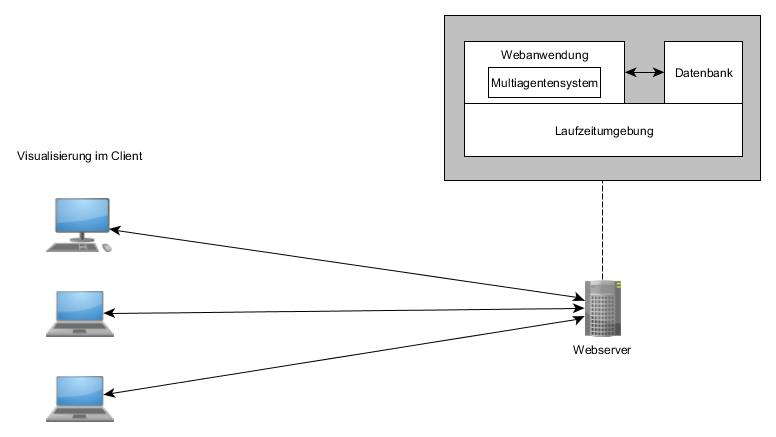
\includegraphics[width=0.8\textwidth]{grobarchitektur.jpg}        GRAFIK FEHLT!
%		\caption{Gesamtarchitektur}
%	\label{Gesamtarchitektur}
%\end{figure} 

